
\FloatBarrier
\section{Система Рёсслера} %  % {{{1 _ROSS_
\label{atu:sect:ross}

\LinkRef{
  ross: ASAU-14. ISDMCI-2011, ISDMCI-2012
  % ~/doc/tex/asau/asau14/atu/atu.tex
}

\subsection{Определение системы и анализ её динамики} %  % {{{2 _ross_task

% TODO original Rossler
Динамическая система Рёсслера~(\ref{atu:eq:rossler})
является в кокой-то мере абстрактной моделью,
описывающей кинетику колебательных и хаотических химических процессов
~\cite{neimark_stoch_chaos_vibro,koltsova_nl_dyn_chem,berje_order_in_chaos,chulichkcov_mm_ml_dyn},
таких как реакция Белоусова-Жаботинского, кристаллизации фосфита свинца и других реакций.


\begin{equation}
\begin{cases}
  \dot{x}  = -y - z  ,  \\
  \dot{y}  = x + a y ,\\
  \dot{z}  = b + z \cdot ( x-c ) .
\end{cases}
\label{atu:eq:rossler}
\end{equation}

Здесь \(x\), \(y\), \(z\) -- переменные состояния системы,
которые соответствуют концентрациям основных реагентов
в моделируемой химической системе.
Соответственно \(a\), \(b\), \(c\) --
параметры, определяющие динамику системы
(в моделируемой системе определяются константами химического равновесия
и концентрациями вспомогательных реагентов).

При моделировании данной системы положим
\(a=0.25\), \(b=1\).
В этом случае параметр \(c\) определяет
тип динамики системы.
Определение значения данного параметра и будет
целью задачи идентификации.

В данной системе нет внешнего входного сигнала \( u(t) \).
Это объясняется тем, что за счет
поддержания постоянных концентраций вспомогательных
компонент, постоянного пополнения исходных веществ
и удаления продуктов реакции система обладает
собственным источником энергии, который обеспечивает
динамику системы и при отсутствии
внешнего воздействия.

Как и другие системы хаотической динамики, система Ресслера
не позволяет построить систему идентификации, основанную
на формировании критерия качества идентификации
как меры близости непосредственных значений выходных сигналов
объекта \( x_0(t) \) и модели \( x_m(t) \).
Более того, сам вид поведения данной системы может значительно изменяться
при малых изменениях параметров, совершая переход от
хаотического к сложно-периодическому и обратно.

При малых значениях параметра (\(c \approx 3 \))
система проявляет регулярную динамику,
совершая колебательное движение вокруг точки
неустойчивого равновесия~(рис.~\ref{atu:f:ross_attractor_0300}).

\begin{figure}[ht!]
\begin{center}
  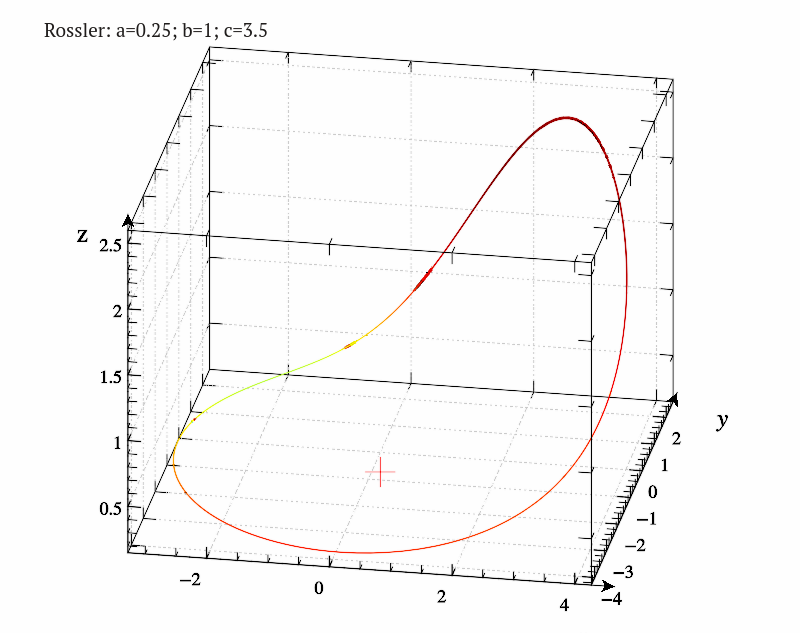
\includegraphics[width=0.49\textwidth]{p/cha/ross/ross0-p_xyz_c=03x50.png}
  \hfill
  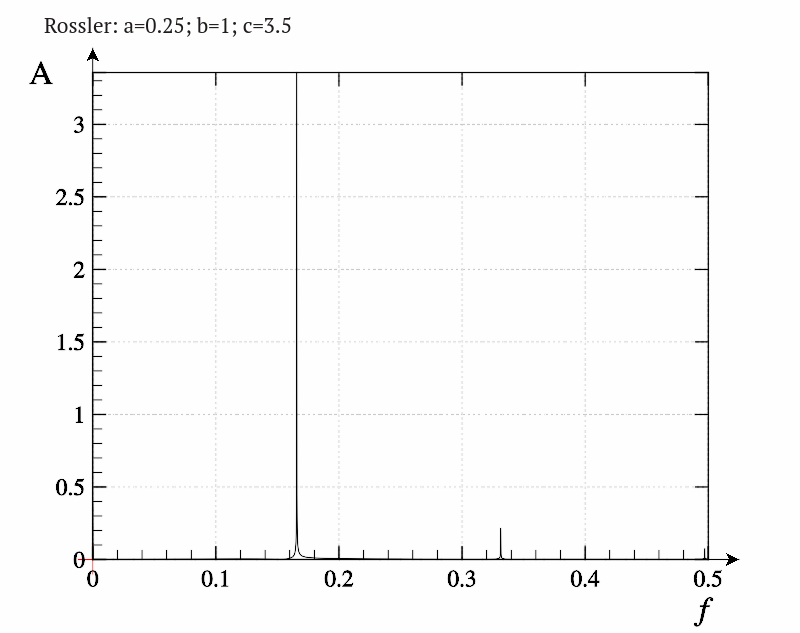
\includegraphics[width=0.49\textwidth]{p/cha/ross/ross_f-p_f_c=03x50.png}
\end{center}
  \caption{Аттрактор и спектр системы Рёсслера (\ref{atu:eq:rossler}) в режиме регулярных колебаний ($c=3.5$)}
\label{atu:f:ross_attractor_0300}
\end{figure}

При увеличении значения параметра \(c\) происходит удвоение периода,
поведение системы становится все более сложным, и в определенном
диапазоне значений параметра система демонстрирует
хаотическую динамику(рис.~\ref{atu:f:ross_attractor_0588}).

\begin{figure}[ht!]
\begin{center}
  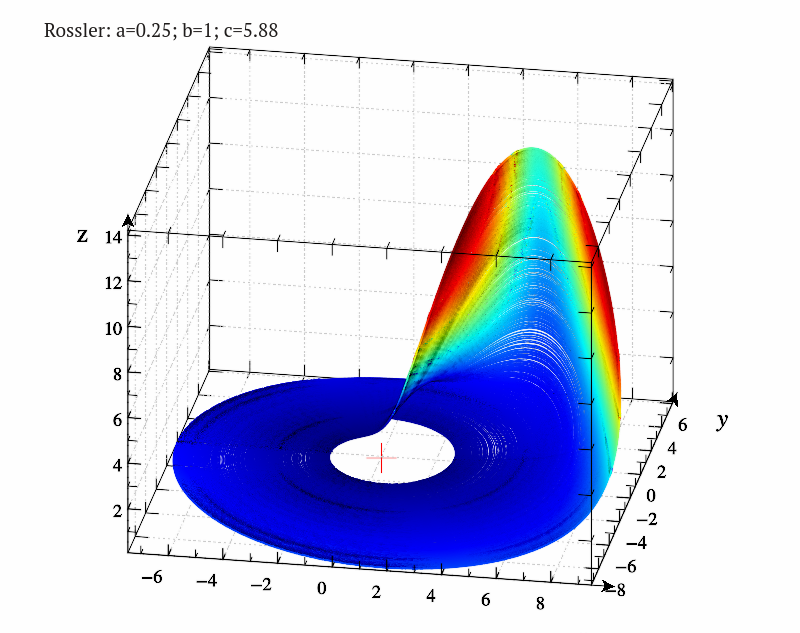
\includegraphics[width=0.49\textwidth]{p/cha/ross/ross0-p_xyz_c=05x88.png}
  \hfill
  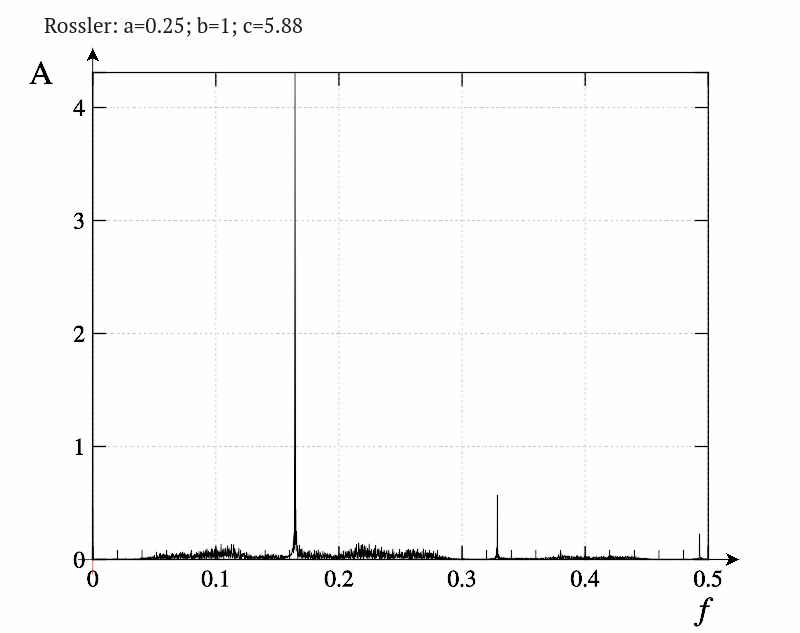
\includegraphics[width=0.49\textwidth]{p/cha/ross/ross_f-p_f_c=05x88.png}
\end{center}
  \caption{Аттрактор и спектр системы Рёсслера (\ref{atu:eq:rossler}) в режиме хаотических колебаний ($c=5.88$)}
\label{atu:f:ross_attractor_0588}
\end{figure}


Прослеживается отличие спектра системы Рёсслера в хаотическом режиме
от аналогичных условий для систем Лоренца. Отличие заключается в том, что
существует ярко выраженный пик, соответствующий базовой частоте,
а области сплошного спектра характеризуются небольшой амплитудой.
При некоторых больших значениях параметра $c$
область сплошного спектра становится более заметной,
однако общая структура спектра остаётся такой же.


При дальнейшем увеличении значения параметра \(c\)
наблюдаются переходы от хаотического к сложно-периодическому
(рис.~\ref{atu:f:ross_attractor_2500})
и  обратно.

\begin{figure}[ht!]
\begin{center}
  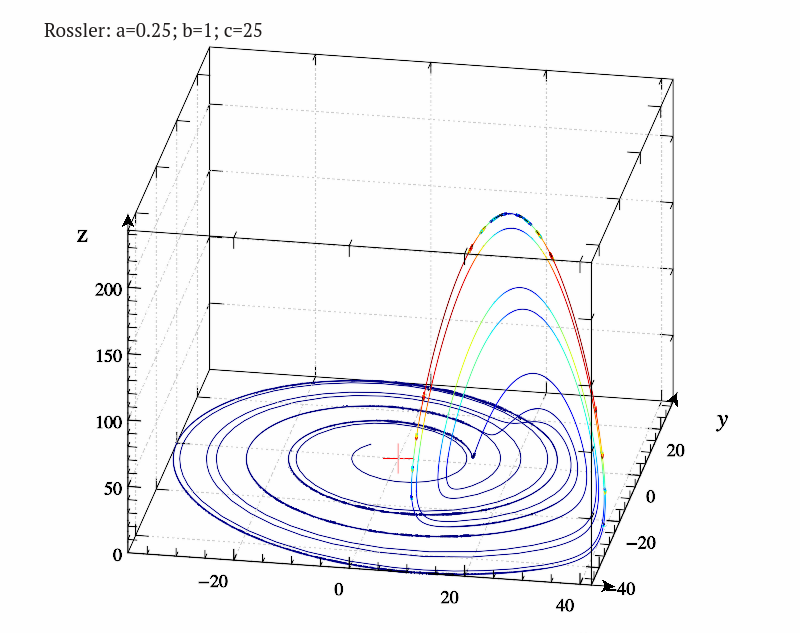
\includegraphics[width=0.49\textwidth]{p/cha/ross/ross0-p_xyz_c=25x00.png}
  \hfill
  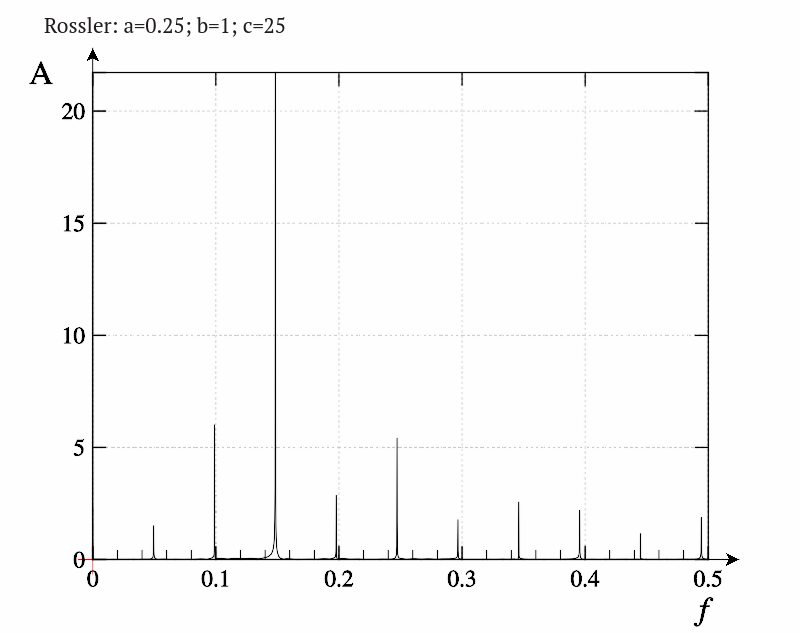
\includegraphics[width=0.49\textwidth]{p/cha/ross/ross_f-p_f_c=25x00.png}
\end{center}
  \caption{Аттрактор и спектр системы Рёсслера (\ref{atu:eq:rossler}) в режиме сложно-периодических колебаний ($c=25.0$)}
\label{atu:f:ross_attractor_2500}
\end{figure}

При этом наблюдается линейчатый спектр. Также при
таких периодах может скачкообразно изменятся
размер области, в которую вписан аттрактор.
В этом смысле система Рёсслера потенциально является более сложной
для идентификации, чем системы Лоренца и ``Sprott A''.

Участки хаотической динамики перемежаются с участками сложно-периодических
колебаний. При этом происходит изменение структуры аттрактора.
Более того, при одном и том же типе динамики может изменяться как структура аттрактора,
так и размер области, в которую он может быть вписан.

% Идентифицируемый параметр:
% $ c \in [2; 50] $, $c_0=5.88$.
%
% Остальные параметры:
% \( a \in (0, 0.35 ) \), $a_0=0.25$,
% \(b \in[0;4] \), $b_0=1$.


% }}}2

\subsection{Анализ и выбор критериев}  % {{{2

Система Рёсслера отличается от уже рассмотренных систем тем,
что соответствующая физическая (или химическая) система
находится в условиях, в которых нет смысла использовать
закон сохранения энергии. Концентрации реагентов,
которые расходуются в реакции, поддерживаются на постоянном уровне
за счёт внешних воздействий. Также считается,
что неиспользуемые продукты реакций удаляются.
Такие свойства дают основания предполагать,
что стандартный набор критериев, который был применён для
систем Лоренца и системы ``Sprott A'', не будет
содержать подходящего критерия. Исходя из формы аттрактора,
содержащего близкие к круговым траектории вблизи плоскости $XY$,
добавим критерий $q_{x^2+y^2}$ к списку рассматриваемых.
Наблюдения за изменением формы аттрактора при увеличении параметра $c$
позволяют заметить, что, в целом, максимальная аппликата также
растёт. Это наблюдение позволяет добавить критерий $q_{z \max{}}$
в число рассматриваемых. Зависимости рассматриваемых критериев от $c$
приведены на рис.~\ref{atu:f:ross_q}.



\begin{figure}[ht!]
\begin{center}
  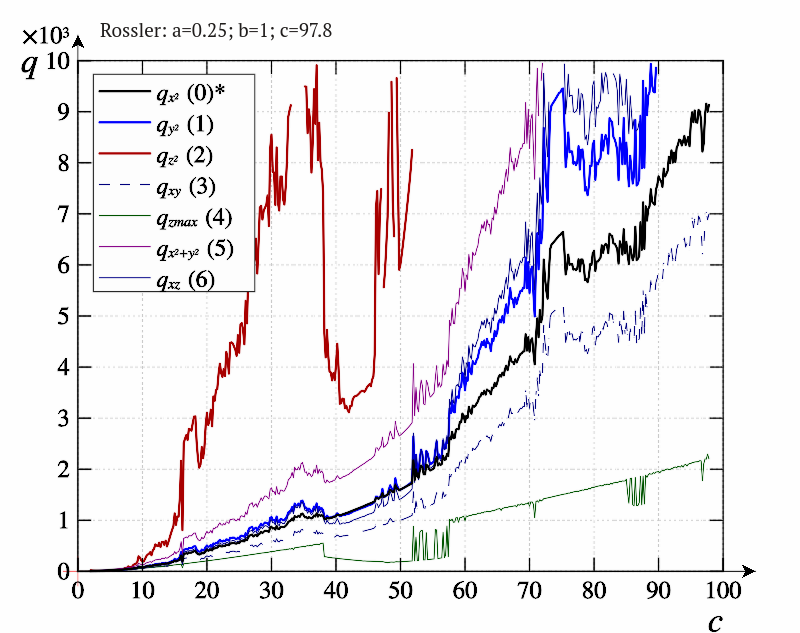
\includegraphics[width=0.49\textwidth]{p/cha/ross/ross_q-p_q.png}
  \hfill
  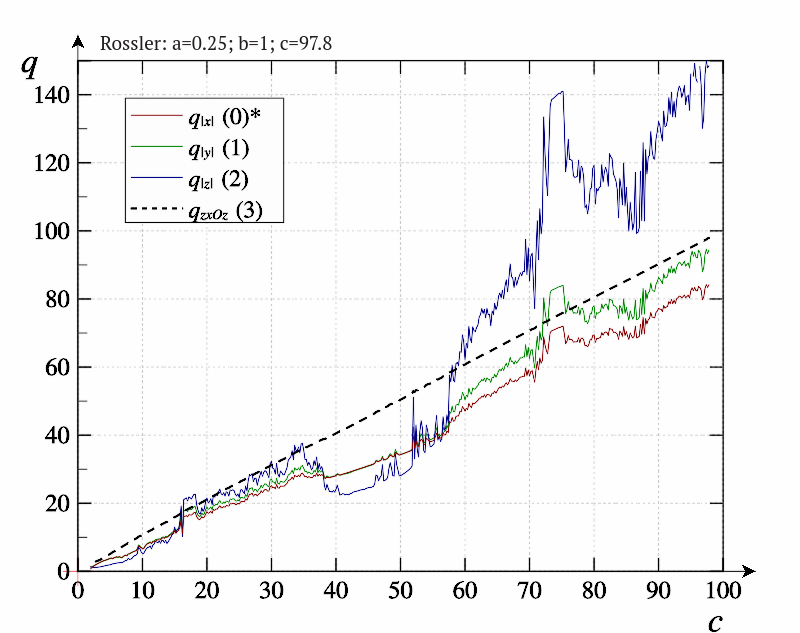
\includegraphics[width=0.49\textwidth]{p/cha/ross/ross_q-p_q1.png}
\end{center}
  \caption{Рассматриваемые критерии для системы Рёсслера}
\label{atu:f:ross_q}
\end{figure}

Как и следовало ожидать, большая часть критериев мало пригодна
для применения в методах идентификации. Несмотря на явные
общие тенденции в поведении графиков, наличие нерегулярных колебаний
не позволяют рассчитывать на приемлемую точность.
Лучшие свойства демонстрирует критерий $q_{z \max{}}$,
график которого содержит сравнительно длинные прямые участки.
Однако, применение этого критерия ограничено одним таким участком,
границы которого зависят от других параметров системы.

Для примера рассмотрим зависимости критерия $q_{x^2}$
от значений двух параметров~(рис.~\ref{atu:f:ross_q_x2_ac_bc}).

\begin{figure}[ht!]
\begin{center}
  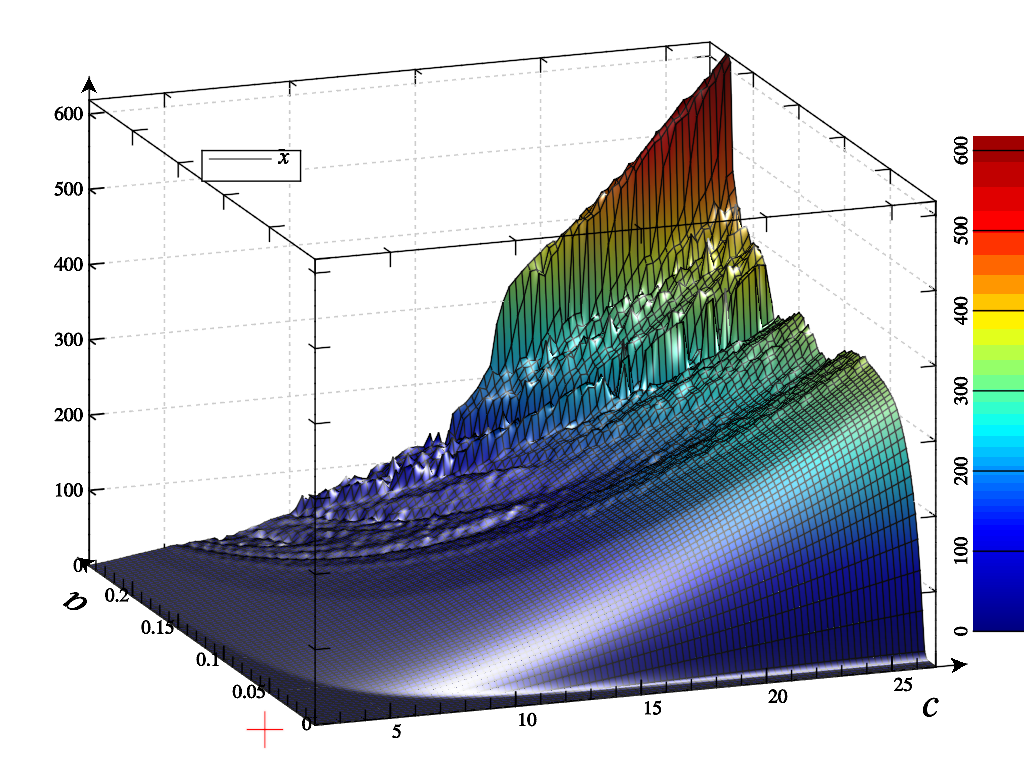
\includegraphics[width=0.49\textwidth]{p/cha/ross/ross_pwr-x_a_c.png}
  \hfill
  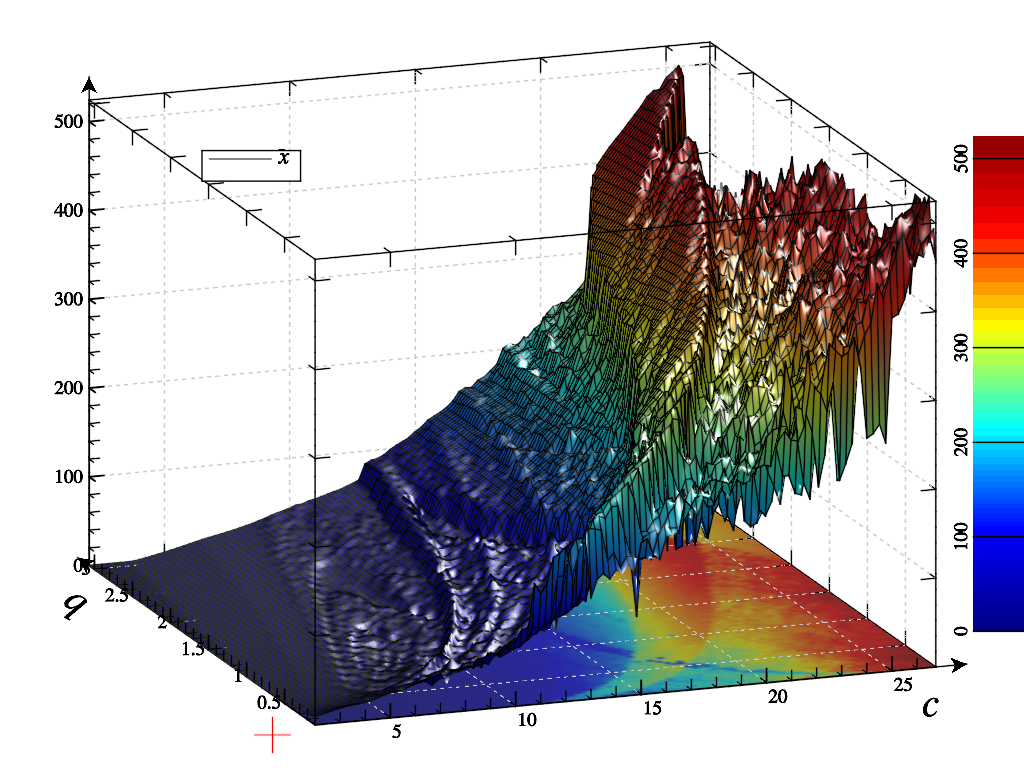
\includegraphics[width=0.49\textwidth]{p/cha/ross/ross_pwr-x_b_c.png}
\end{center}
  \caption{Зависимости $q_{x^2}(a,c)$ и  $q_{x^2}(b,c) $ для системы Рёсслера}
\label{atu:f:ross_q_x2_ac_bc}
\end{figure}

Сложная и изрезанная структура полученных поверхностей
свидетельствует не только о практически невозможной идентификации одновременно двух параметров,
но и о том, что достаточно малые ошибки о определении одного из них
приводят к существенным ошибкам идентификации другого.

Зависимости $q_{z \max{}}(a,c)$ и  $q_{z \max{}}(b,c) $
(рис.~\ref{atu:f:ross_q_zmax_ac_bc}) построенные для
области параметров, для которой не наблюдается существенное изменение
поведения критерия, показывает лучшие результаты. Однако,
даже в этой области происходят резкие ``провалы'' графика.
Такое поведение может и не привести в существенным ошибкам идентификации.
Тем не менее, при попадании одной из моделей в область ``провала''
процесс идентификации может быть нарушен.

\begin{figure}[ht!]
\begin{center}
  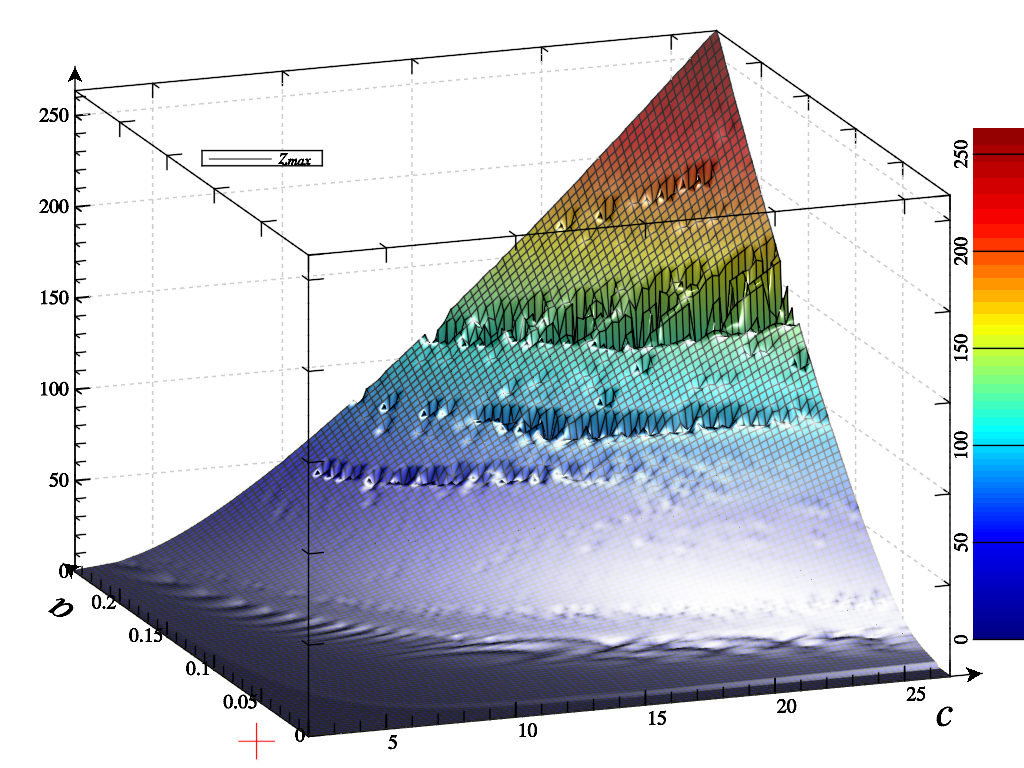
\includegraphics[width=0.49\textwidth]{p/cha/ross/ross_zmax_a_c.png}
  \hfill
  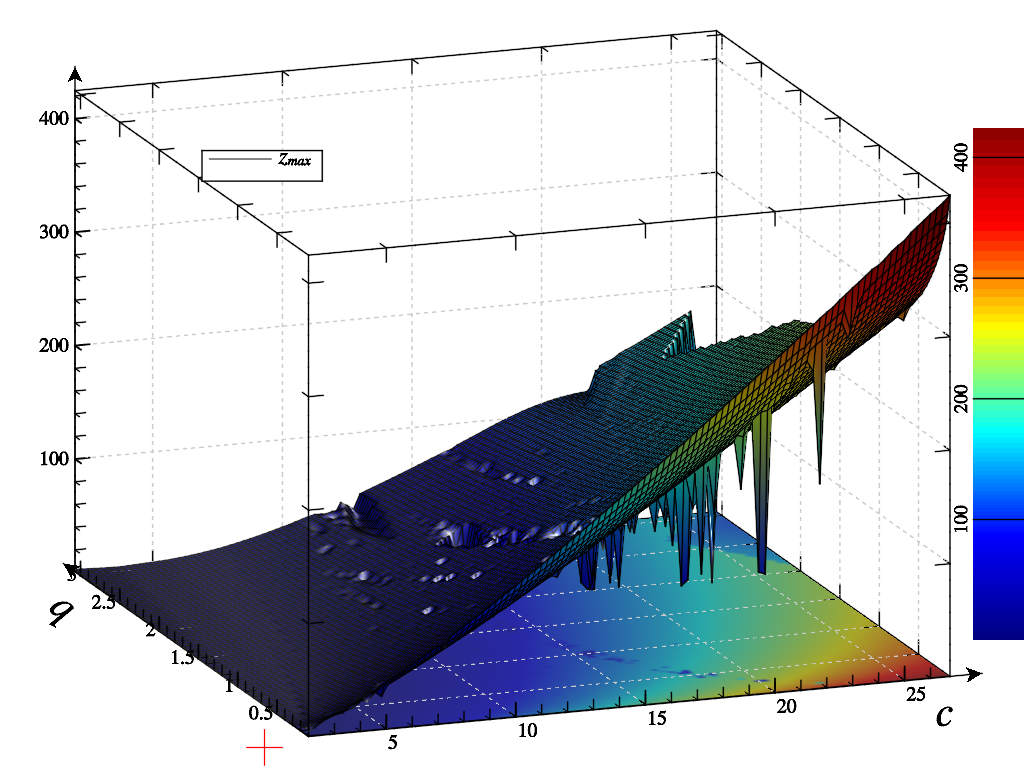
\includegraphics[width=0.49\textwidth]{p/cha/ross/ross_zmax_b_c.png}
\end{center}
  \caption{Зависимости $q_{z \max{}}(a,c)$ и  $q_{z \max{}}(b,c) $ для системы Рёсслера}
\label{atu:f:ross_q_zmax_ac_bc}
\end{figure}

Попробуем вывести более пригодный для задачи идентификации критерий,
исходя из вида системы~(\ref{atu:eq:rossler}).
Непосредственно параметр $c$ входит только в последнее уравнение системы.
Так как рассматриваются только режимы, проявляющие устойчивою по Пуассону динамику,
то при усреднении на большом интервале времени левая часть стремится к нулю.
В правой части есть два параметра: $c$ и $b$.
Даже для условий усреднения нет возможности определить оба,
но для идентификации $c$ введём следующий вид критерия:
%
\begin{equation}
  q_{xzOz} =
  \frac{ \overline{xz}}{ \overline{z}}.
  \label{atu:eq:ross_qzxOz}
\end{equation}

При фиксированных параметрах $a$ и $b$ график $q_{xzOz}(c)$
представляет собой близкую к линейной
зависимость~(рис.~\ref{atu:f:ross_q}, правый график, пунктирная кривая).
Однако, применение этого критерия приводит к определённым трудностям.
Прежде всего, наличие дробной зависимости требует отдельного анализа
знаменателя. Из анализа аттрактора системы известно, что $z>0 \; \forall \; t > 0$,
то есть знаменатель в ноль не обращается. При этом вид
зависимости $z(t)$ характеризуется резкими всплеками,
между которыми находятся области, в которых $z \approx 0 $,
что может привести к значительным всплескам в значении критерия.
Однако, эта же величина $z$ входит и в числитель как множитель,
и если метод и параметры устреднения в числителе и знаменателе
одинаковые, то возмущения критерия будут ограниченными.


% }}}2

\subsection{Тестовая задача идентификации для системы Рёсслера}  % {{{2

Для синтеза системы идентификации был выбрана группа методов ``ql3rlWvnAAW'',
критерий $q_{xzOz}$.
Используемые значения параметров: $a=0.25$, $b=1$, $ c \in [3, 40 ]$.
Прежде всего, рассмотрим процесс идентификации
в квазистационарном случае,
при медленном изменении параметра~(\ref{atu:eq:po_t_ramp}), $p_0=10$, $U_p=20$.
Динамика агентов и различных определений $p_\mathrm{id}$
представлена на рис.~\ref{atu:f:ross_id_ramp}.


\begin{figure}[ht!]
\begin{center}
  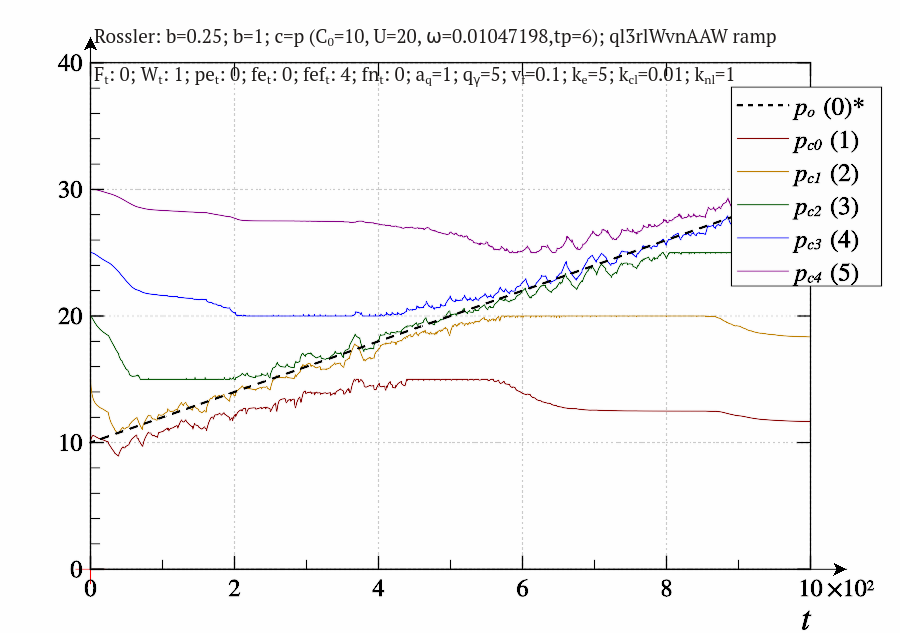
\includegraphics[width=0.49\textwidth]{p/cha/ross/ross_id-p_t_pi_ql3rlWvnAAW_ramp.png}
  \hfill
  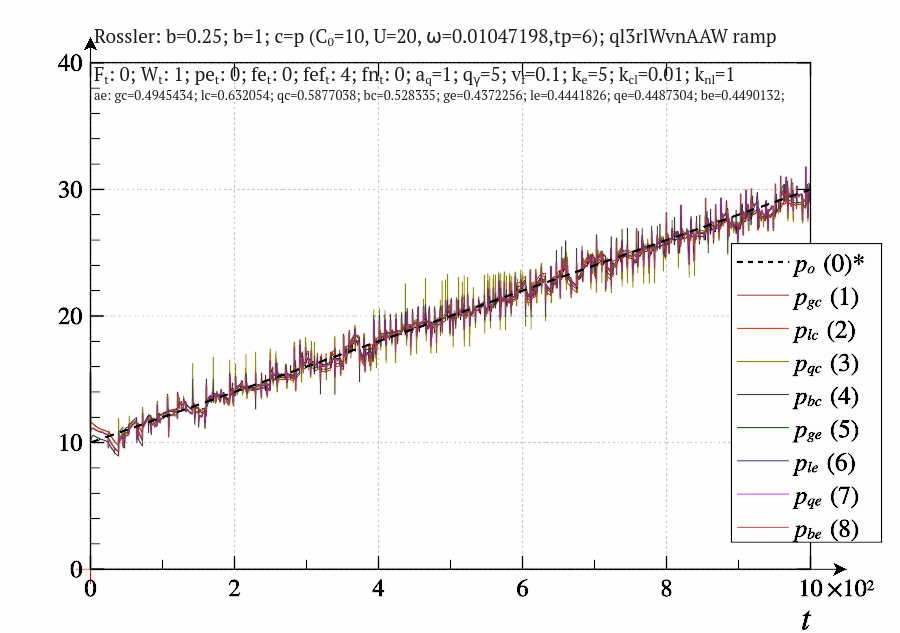
\includegraphics[width=0.49\textwidth]{p/cha/ross/ross_id-p_t_p_ql3rlWvnAAW_ramp.png}
\end{center}
  \caption{Динамика агентов и идентифицируемого значения для системы Рёсслера при условии (\ref{atu:eq:po_t_ramp})}
\label{atu:f:ross_id_ramp}
\end{figure}

Графики динамики агентов показывают, что наблюдается корректное
``сопровождение'' агентами идентифицируемого параметра, за исключением
небольшого начального участка, на котором усреднение критерия
на даёт корректных результатов. Все зависимости $p_\mathrm{id}(4)$
имеют практически неотличимую динамику, хорошее приближение идентифицируемого параметра.
При этом наблюдаются незначительные, но резкие ``всплески'',
вызванные аналогичным явлением для критерия.
Хорошим признаком является тот, что не наблюдается областей,
в которых процесс идентификации нарушается или заметно теряет точность.

Рассмотрим динамку процесса идентификации
(рис.~\ref{atu:f:ross_id_sign})
в том случае,
если идентифицируемый параметр претерпевает
резкие скачки~(\ref{atu:eq:po_t_sign}), $p_0=21$, $U_p=7$, $\omega_{in}=0.01047$.

\begin{figure}[ht!]
\begin{center}
  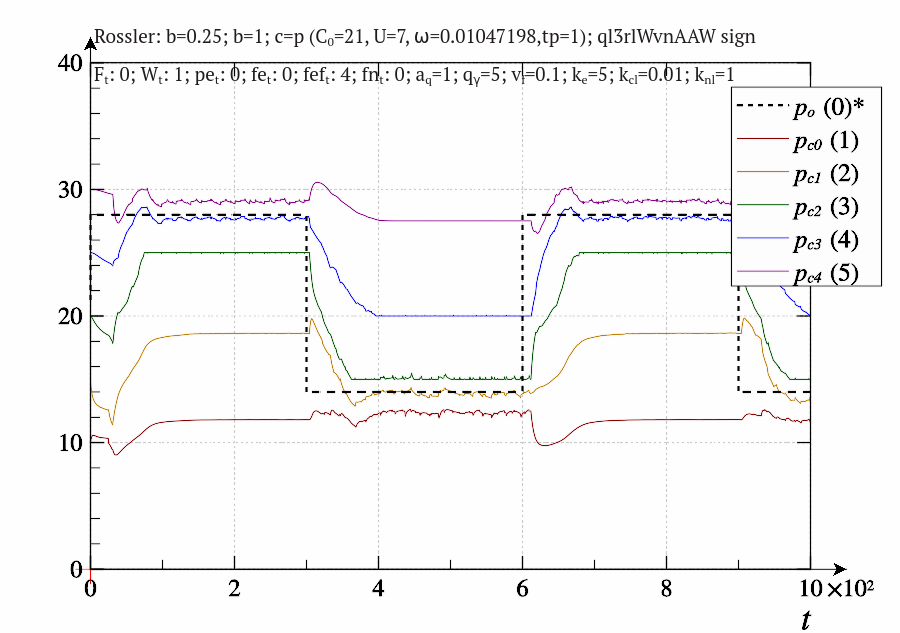
\includegraphics[width=0.49\textwidth]{p/cha/ross/ross_id-p_t_pi_ql3rlWvnAAW_sign.png}
  \hfill
  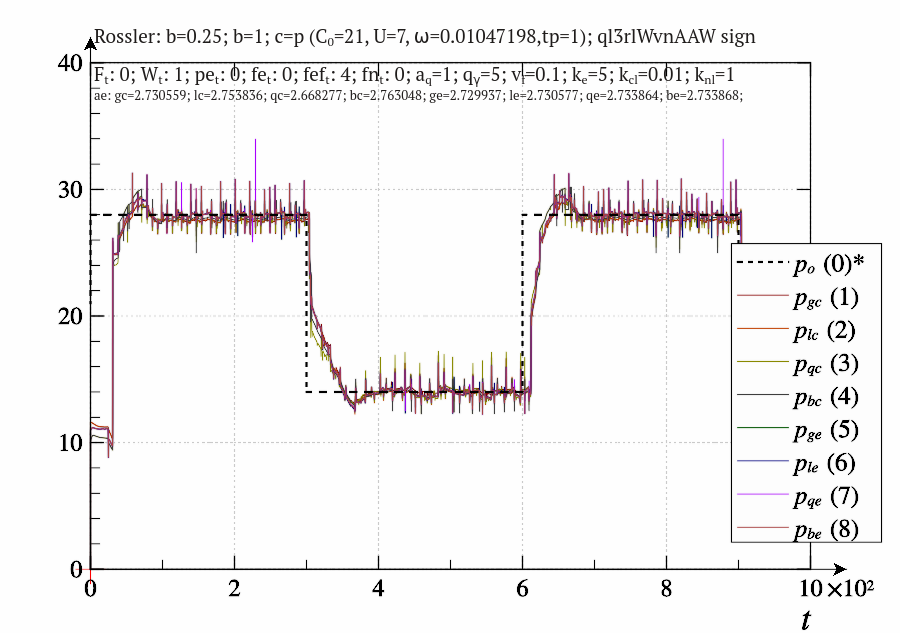
\includegraphics[width=0.49\textwidth]{p/cha/ross/ross_id-p_t_p_ql3rlWvnAAW_sign.png}
\end{center}
  \caption{Динамика агентов и идентифицируемого значения для системы Рёсслера при условии (\ref{atu:eq:po_t_sign})}
\label{atu:f:ross_id_sign}
\end{figure}

Помимо общей работоспособности метода идентификации следует отметить,
что в данном случае все рассматриваемые способы определения $p_\mathrm{id}$
дают практически неразличимые результаты.

На рис.~\ref{atu:f:ross_id_sin}
представлены аналогичные результаты,
но в случае более плавного изменения параметра~(\ref{atu:eq:po_t_sin}), при прочих равных.


\begin{figure}[ht!]
\begin{center}
  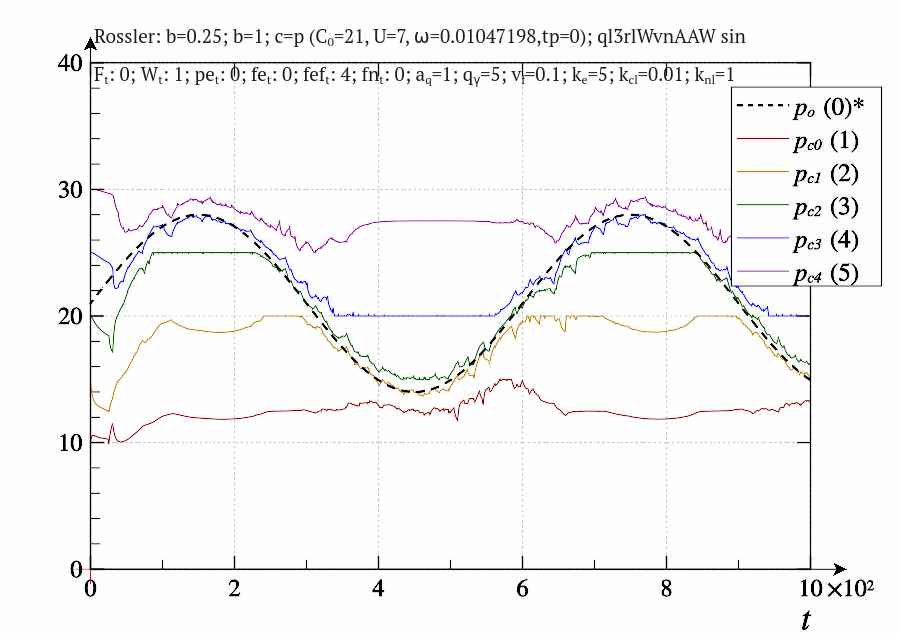
\includegraphics[width=0.49\textwidth]{p/cha/ross/ross_id-p_t_pi_ql3rlWvnAAW_sin.png}
  \hfill
  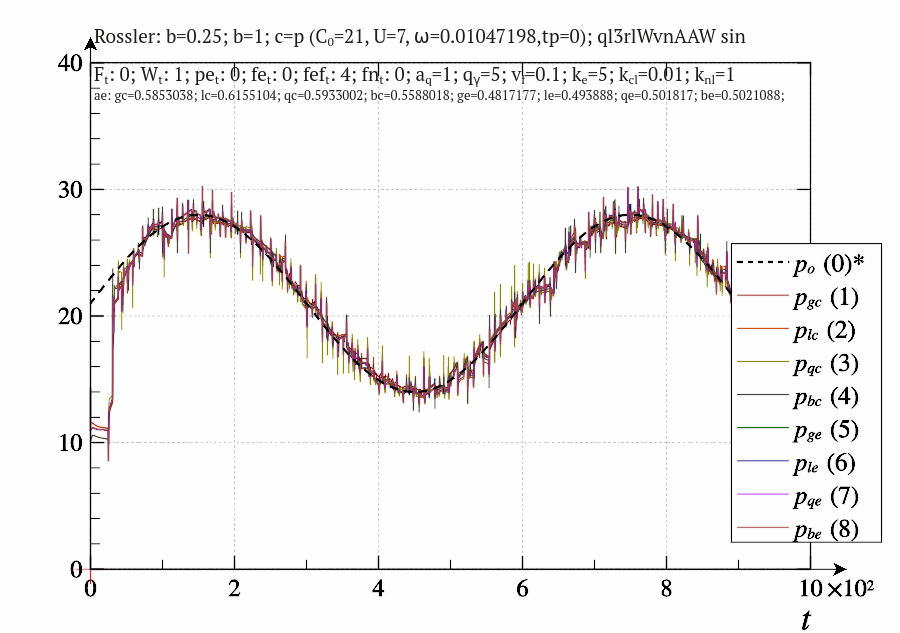
\includegraphics[width=0.49\textwidth]{p/cha/ross/ross_id-p_t_p_ql3rlWvnAAW_sin.png}
\end{center}
  \caption{Динамика агентов и идентифицируемого значения для системы Рёсслера при условии (\ref{atu:eq:po_t_sin})}
\label{atu:f:ross_id_sin}
\end{figure}

Принципиальных отличий не выявлено, средняя ошибка идентификации в этом
случае ниже, что достаточно очевидно.


% }}}2

\subsection{Влияние параметров системы идентификации на ошибку идентификации для системы Рёсслера}  % {{{2

Рассмотрим влияние параметров системы идентификации.
Для рассматриваемой системы выбор правильного значения $a_q$
особенно важен, ввиду наличия резких импульсов в значении критерия.
Характерных вид такой зависимости представлен на рис.~\ref{atu:f:ross_q_t}.

\begin{figure}[ht!]
\begin{center}
  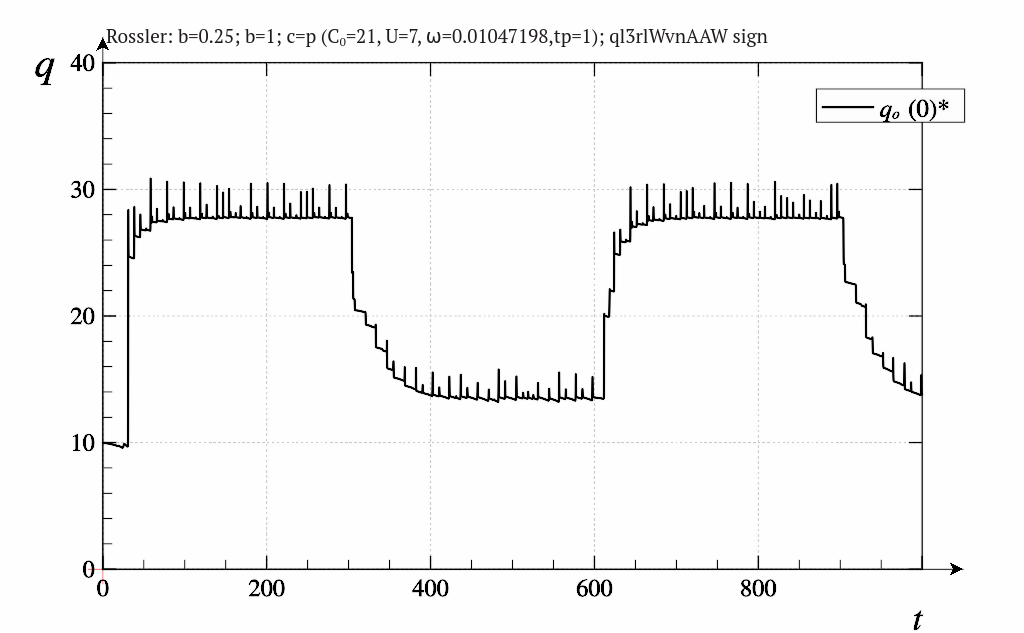
\includegraphics[width=0.49\textwidth]{p/cha/ross/ross_id-p_t_q_ql3rlWvnAAW_sign.png}
  \hfill
  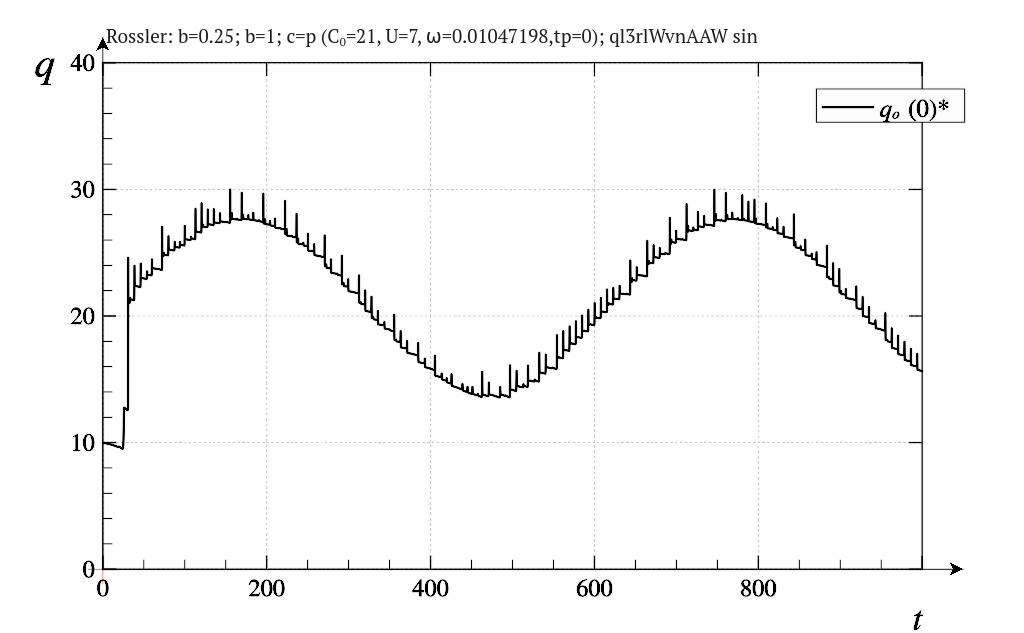
\includegraphics[width=0.49\textwidth]{p/cha/ross/ross_id-p_t_q_ql3rlWvnAAW_sin.png}
\end{center}
  \caption{Характерных вид зависимостей $q_{xzOz}(t)$ для системы Рёсслера}
\label{atu:f:ross_q_t}
\end{figure}

Несмотря на наличие таких импульсов,
общий вид зависимости ошибки идентификации
остаётся неизменным~(рис.~\ref{atu:f:ross_e_a_q}).
Так как большинство методов определения $p_\mathrm{id}$
дают близкие результаты, на на этом и последующих графиках
ограничимся пятью. Рост ошибки идентификации при $a_q \to 0$
обусловлен тем, что избыточные фильтрующие свойства критерия
не позволяют не только отреагировать, но и заметить изменение динамики системы.
Рост в правой части графика, как и в предыдущих тестовых задачах,
обусловлен недостаточным временем усреднения критерия.

\begin{figure}[ht!]
\begin{center}
  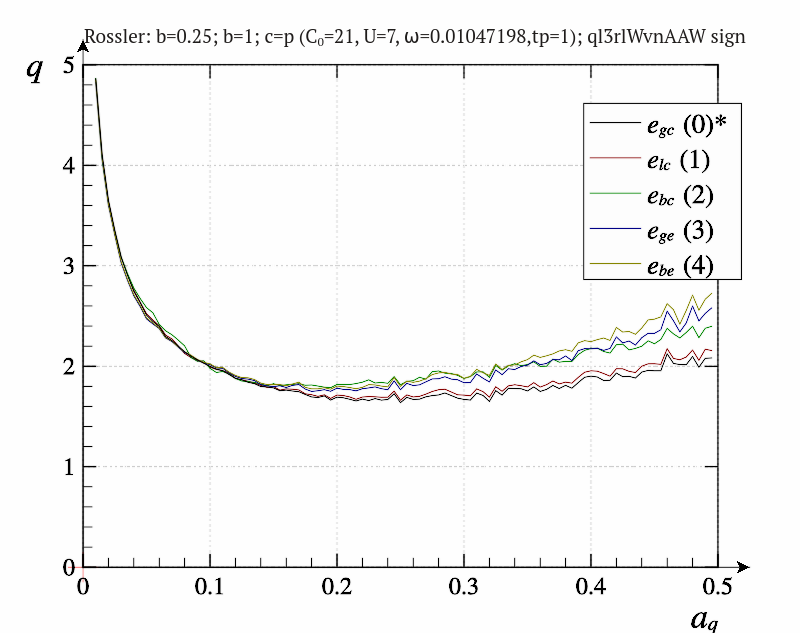
\includegraphics[width=0.49\textwidth]{p/cha/ross/ross_id-p_a_q_ql3rlWvnAAW_sign.png}
  \hfill
  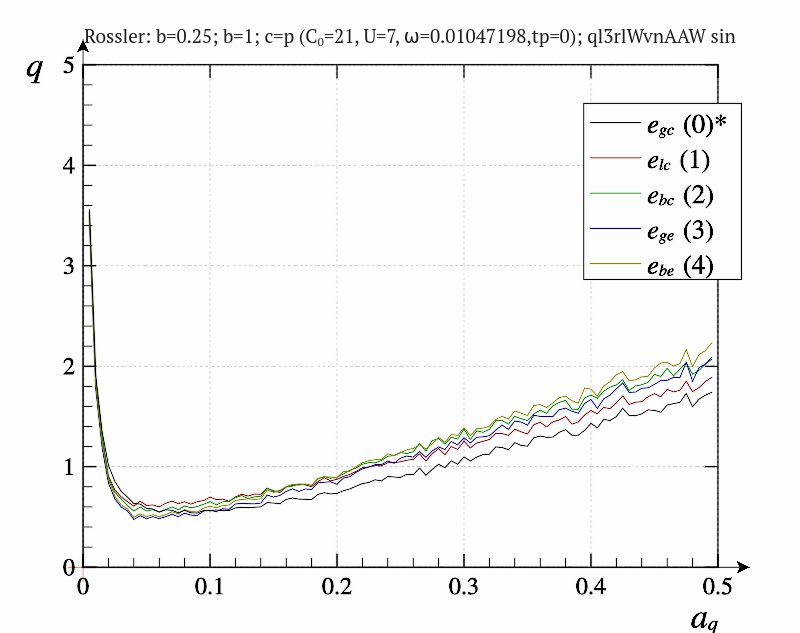
\includegraphics[width=0.49\textwidth]{p/cha/ross/ross_id-p_a_q_ql3rlWvnAAW_sin.png}
\end{center}
  \caption{Зависимости $\bar{e}(a_q)$ для системы Рёсслера}
\label{atu:f:ross_e_a_q}
\end{figure}

Следующий параметр, влияющий на свойства системы идентификации --- $q_\gamma$.
Для семейства методов ``ql3rlWvnAAW'' он применяется дважды.
Первый раз, в составе значения $W$, он определяет
динамику одного агента. Второй раз --- задаёт уровень влияния агента
на уровне координатора. В отличие от методов ``Fq\ldots''
этот параметр не участвует при определении агентом величины $p_e$.
Полученные зависимости $\bar{e}(q_\gamma)$
представлены на рис.~\ref{atu:f:ross_e_q_gamma}.

\begin{figure}[ht!]
\begin{center}
  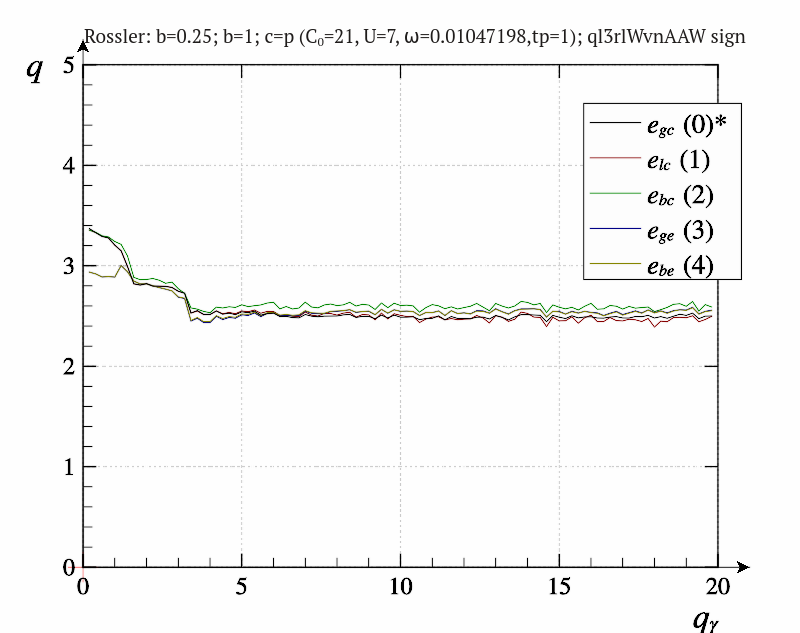
\includegraphics[width=0.49\textwidth]{p/cha/ross/ross_id-p_q_gamma_ql3rlWvnAAW_sign.png}
  \hfill
  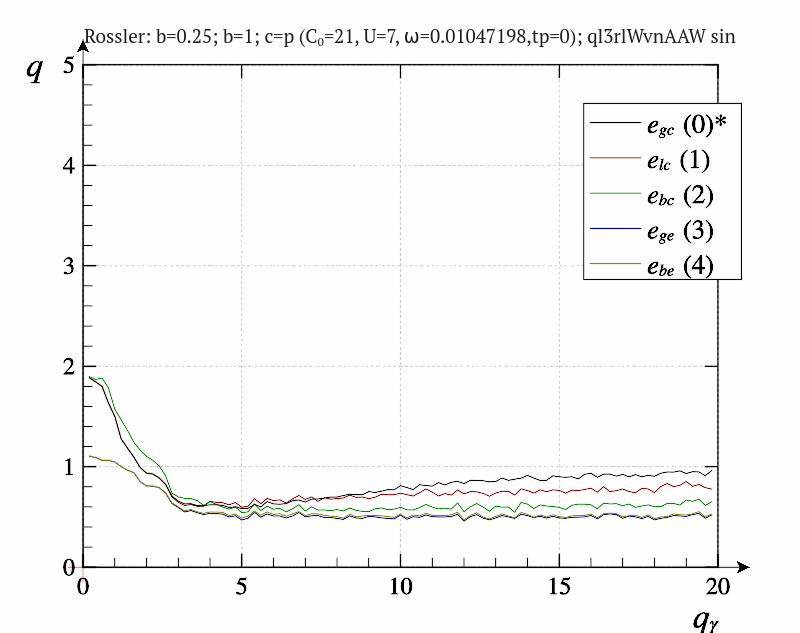
\includegraphics[width=0.49\textwidth]{p/cha/ross/ross_id-p_q_gamma_ql3rlWvnAAW_sin.png}
\end{center}
  \caption{Зависимости $\bar{e}(q_\gamma)$ для системы Рёсслера}
\label{atu:f:ross_e_q_gamma}
\end{figure}

Оба графика демонстрируют увеличение ошибки идентификации при избыточной чувствительности,
т.е. при $q_\gamma \to 0 $.
Однако в дальнейшем поведение графиков различаются. Если
параметр изменяется резко, что ошибки идентификации, связанные с
недостаточной чувствительностью, становятся малыми, по сравнению с ошибками,
обусловленными
ограниченной скоростью изменения критерия, и зависимость от $q_\gamma$
практически отсутствует. При менее ярко выраженной динамке изменения параметра,
появляется как увеличение ошибки из-за недостаточной чувствительности,
так и различие между применяемыми поисковыми координаторами методов.
В первую очередь растёт ошибка идентификации у методов, использующих $p_c$,
во вторую --- у методов, использующих ``глобальные'' оценки.
Но в целом, если исключить область избыточной чувствительности,
влияние этого параметра незначительно, что обусловлено
адаптационными свойствами метода.
Метод ql3rlWvnleW менее других теряет точность при росте чувствительности.

Влияние параметра $v_f$ для методов, использующих ансамбль агентов,
прежде всего обуславливает динамику точной настройки параметра,
а не скорость реакции на резкие изменения параметра.
Поэтому правый график соответствующих зависимостей
(рис.~\ref{atu:f:ross_e_v_f}), показывает
более значительное влияние этого параметра.


\begin{figure}[ht!]
\begin{center}
  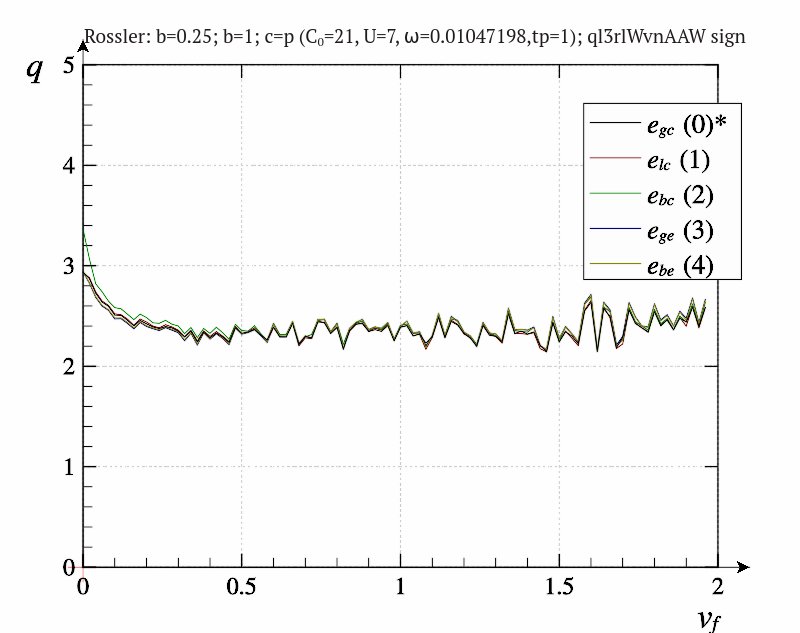
\includegraphics[width=0.49\textwidth]{p/cha/ross/ross_id-p_v_f_ql3rlWvnAAW_sign.png}
  \hfill
  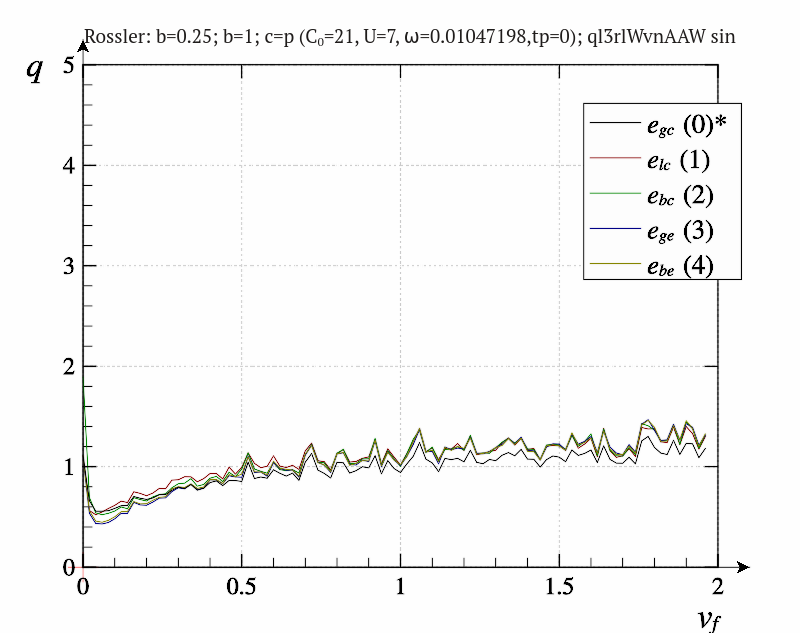
\includegraphics[width=0.49\textwidth]{p/cha/ross/ross_id-p_v_f_ql3rlWvnAAW_sin.png}
\end{center}
  \caption{Зависимости $\bar{e}(v_f)$ для системы Рёсслера}
\label{atu:f:ross_e_v_f}
\end{figure}


Левый график свидетельствует о том, что при скачкообразном изменении параметра
оправданной становится большая скорость перемещения агентов,
несмотря на уменьшение точности из-за избыточного рысканья агентов.
Следует отметить, что в данном примере перемещение агентов ограничено.
Без этого ограничения при росте $v_f$ наблюдается нарушение устойчивости поиска.

Влияние коэффициента $k_e$ (рис.~\ref{atu:f:ross_e_k_e})
в какой-то мере схоже с влиянием коэффициента $v_f$.
Отличие заключается в том, что $k_e$ влияет не только на скорость перемещения агентов,
но на их равновесную конфигурацию.

\begin{figure}[ht!]
\begin{center}
  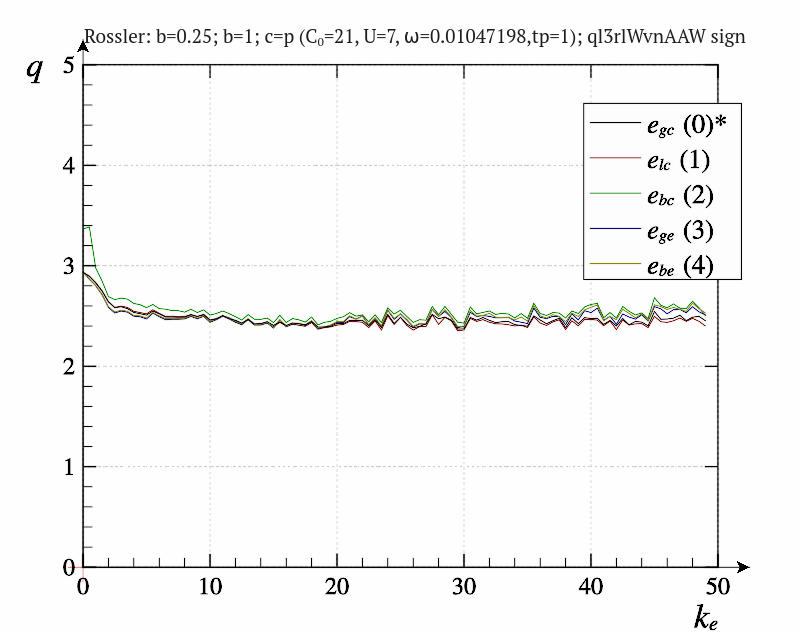
\includegraphics[width=0.49\textwidth]{p/cha/ross/ross_id-p_k_e_ql3rlWvnAAW_sign.png}
  \hfill
  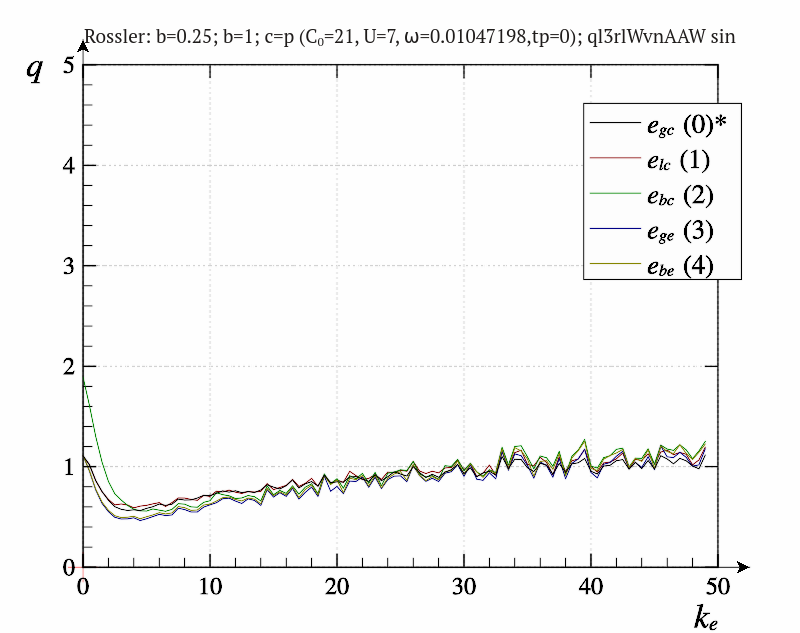
\includegraphics[width=0.49\textwidth]{p/cha/ross/ross_id-p_k_e_ql3rlWvnAAW_sin.png}
\end{center}
  \caption{Зависимости $\bar{e}(k_e)$ для системы Рёсслера}
\label{atu:f:ross_e_k_e}
\end{figure}

Как и для предыдущего параметра, влияние этого коэффициента
более значительно при плавном изменении параметра.
И опять же, без искусственного ограничения подвижности агентов
высокие величины $k_e$ приводят к потере устойчивости поиска.

Влияние параметра $k_{nl}$ (рис.~\ref{atu:f:ross_e_k_nl})
отображает свойства множества агентов как ансамбля.

\begin{figure}[ht!]
\begin{center}
  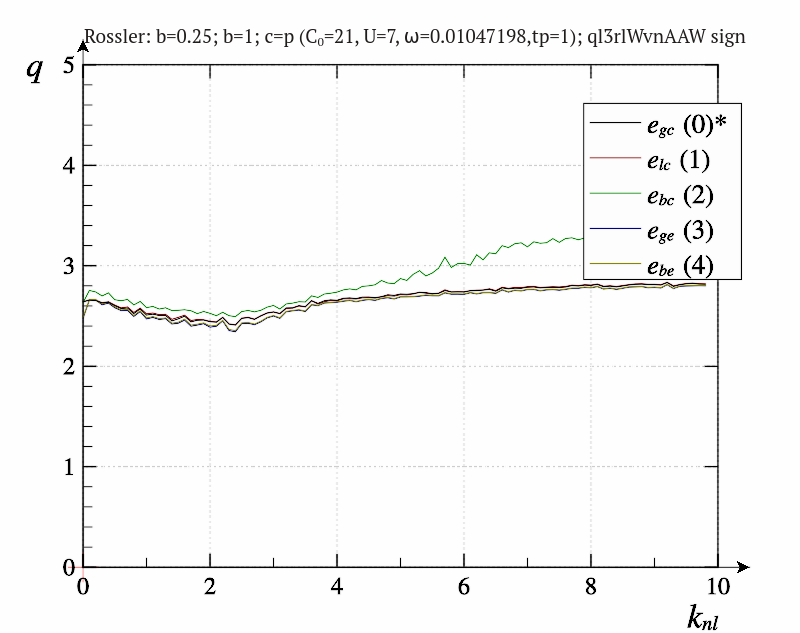
\includegraphics[width=0.49\textwidth]{p/cha/ross/ross_id-p_k_nl_ql3rlWvnAAW_sign.png}
  \hfill
  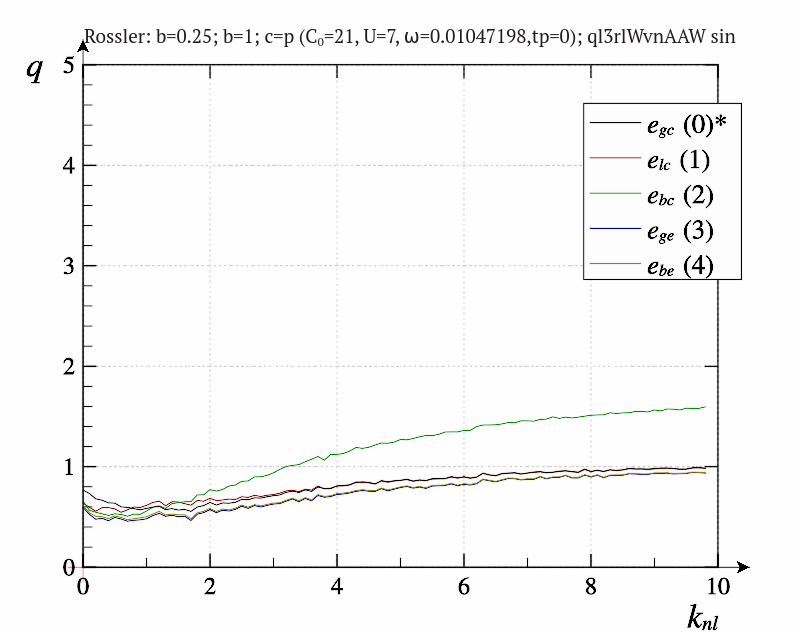
\includegraphics[width=0.49\textwidth]{p/cha/ross/ross_id-p_k_nl_ql3rlWvnAAW_sin.png}
\end{center}
  \caption{Зависимости $\bar{e}(k_{nl})$ для системы Рёсслера}
\label{atu:f:ross_e_k_nl}
\end{figure}

Малые значения величины $k_{nl}$ приводят к тому, что движение
агентов становится практически независимым, при этом конфигурация
агентов вблизи искомого значения далека от оптимальной.
И наоборот, увеличение $k_{nl}$ превращает ансамбль в сетку,
с неизбежным ростом ошибки идентификации.

Наличие искусственных ограничений на перемещения агентов
приводит к тому, что влияние коэффициента $k_{cl}$
становится минимальным (рис.~\ref{atu:f:ross_e_k_cl}).

\begin{figure}[ht!]
\begin{center}
  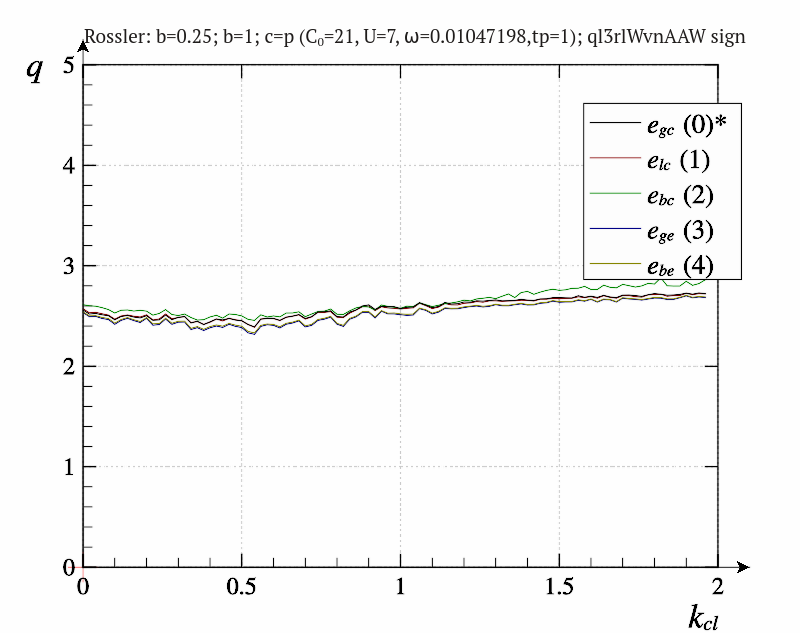
\includegraphics[width=0.49\textwidth]{p/cha/ross/ross_id-p_k_cl_ql3rlWvnAAW_sign.png}
  \hfill
  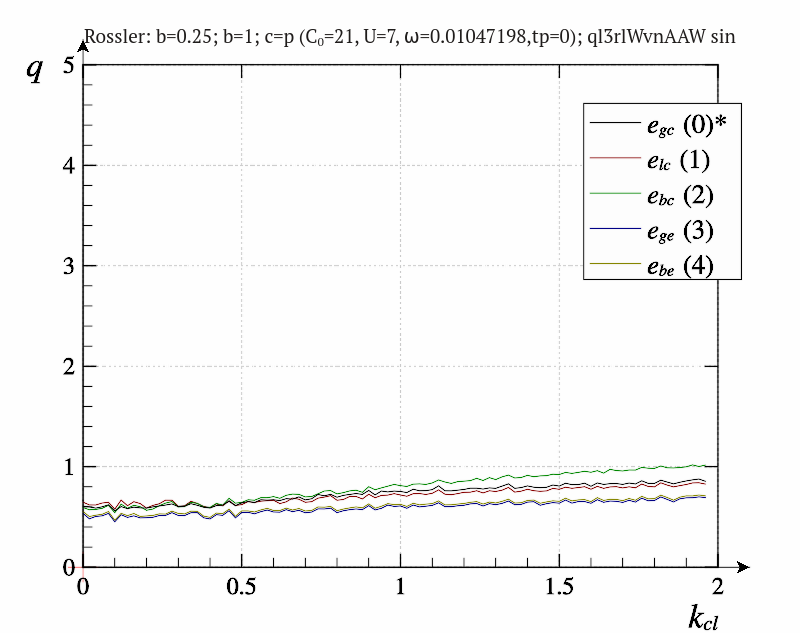
\includegraphics[width=0.49\textwidth]{p/cha/ross/ross_id-p_k_cl_ql3rlWvnAAW_sin.png}
\end{center}
  \caption{Зависимости $\bar{e}(k_{cl})$ для системы Рёсслера}
\label{atu:f:ross_e_k_cl}
\end{figure}

Более того, при плавном изменении параметра его введение только ухудшает
качество идентификации, создавая дополнительную неравномерность в распределении
агентов. При скачкообразном изменении идентифицируемого параметра
несущественное улучшение связано с увеличением расстояния между агентами,
и более быстрой реакцией на скачок.


% }}}2




\subsection{Выводы}  % {{{2

Результаты моделирования
процессов идентификации параметра ``$c$''
системы Рёсслера,
позволяют в сделать следующие выводы:

\begin{itemize}

  \item
    Стандартный набор критериев имеет для этой системы
    весьма ограниченное применение.

  \item
    Использование критерия $q_{xzOz}$
    позволяет построить работоспособную систему идентификации.

  \item
    Группа методов ql3rlWvnAAW показала свою хорошую работоспособность,
    а скорость идентификации при этом в первую очередь определяется
    динамикой критерия.

  \item
    Параметры самой системы идентификации могут изменяться в достаточно широких
    пределах без существенного увеличения ошибки идентификации.

\end{itemize}


% }}}2


% }}}1

% vim: fdm=marker foldlevel=1 foldignore="%#" fdc=4 ft=tex
